% ==== Document Class & Packages =====
\documentclass[12pt,hidelinks]{article}
	\usepackage[explicit]{titlesec}
	\usepackage{titletoc}
	\usepackage{tocloft}
	\usepackage{charter}
	\usepackage[many]{tcolorbox}
	\usepackage{amsmath}
	\usepackage{graphicx}
	\graphicspath{{images/}}
	\usepackage{listings}
	\usepackage{xcolor}
	\usepackage{tikz,lipsum,lmodern}
	\usetikzlibrary{calc}
	\usepackage[english]{babel}
	\usepackage{fancyhdr}
	\usepackage{mathrsfs}
	\usepackage{empheq}
	\usepackage{fourier}% change to lmodern if fourier is no available
	\usepackage{wrapfig}
	\usepackage{fancyref}
	\usepackage{hyperref}
	\usepackage{cleveref}
	\usepackage{listings}
	\usepackage{varwidth}
	\usepackage{longfbox}
	\usepackage{geometry}
	\usepackage{marginnote}
	\tcbuselibrary{theorems}
	\tcbuselibrary{breakable, skins}
	\tcbuselibrary{listings, documentation}
	\geometry{
		a4paper,
		left=33mm,
		right=33mm,
		top=20mm}
% ========= Path to images ============
%   - Direct the computer on the path 
% 	  to the folder containg the images
% =====================================
\graphicspath{{./images/}}
% ============= Macros ================
\newcommand{\fillin}{\underline{\hspace{.75in}}{\;}}
\newcommand{\solution}{\textcolor{mordantred19}{Solution:}}
\setlength{\parindent}{0pt}
\addto{\captionsenglish}{\renewcommand*{\contentsname}{Table of Contents}}
\linespread{1.2}
% ======== Footers & Headers ==========
\cfoot{\thepage}
\chead{}\rhead{}\lhead{}
% =====================================
\renewcommand{\thesection}{\arabic{section}}
\newcommand\sectionnumfont{% font specification for the number
	\fontsize{380}{130}\color{myblueii}\selectfont}
\newcommand\sectionnamefont{% font specification for the name "PART"
	\normalfont\color{white}\scshape\small\bfseries }
% ============= Colors ================
% ----- Red -----
\definecolor{mordantred19}{rgb}{0.68, 0.05, 0.0}
% ----- Blue -----
\definecolor{st.patrick\'sblue}{rgb}{0.14, 0.16, 0.48}
\definecolor{teal}{rgb}{0.0, 0.5, 0.5}
\definecolor{beaublue}{rgb}{0.74, 0.83, 0.9}
\definecolor{mybluei}{RGB}{0,173,239}
\definecolor{myblueii}{RGB}{63,200,244}
\definecolor{myblueiii}{RGB}{199,234,253}
% ---- Yellow ----
\definecolor{blond}{rgb}{0.98, 0.94, 0.75}
\definecolor{cream}{rgb}{1.0, 0.99, 0.82}
% ----- Green ------
\definecolor{emerald}{rgb}{0.31, 0.78, 0.47}
\definecolor{darkspringgreen}{rgb}{0.09, 0.45, 0.27}
% ---- White -----
\definecolor{ghostwhite}{rgb}{0.97, 0.97, 1.0}
\definecolor{splashedwhite}{rgb}{1.0, 0.99, 1.0}
% ---- Grey -----
\definecolor{whitesmoke}{rgb}{0.96, 0.96, 0.96}
\definecolor{lightgray}{rgb}{0.92, 0.92, 0.92}
\definecolor{floralwhite}{rgb}{1.0, 0.98, 0.94}
% ========= Part Format ==========
\titleformat{\section}
{\normalfont\huge\filleft}
{}
{20pt}
{\begin{tikzpicture}[remember picture,overlay]
	\fill[myblueiii] 
	(current page.north west) rectangle ([yshift=-13cm]current page.north east);   
\node[
	fill=mybluei,
	text width=2\paperwidth,
	rounded corners=6cm,
	text depth=18cm,
	anchor=center,
	inner sep=0pt] at (current page.north east) (parttop)
	{\thepart};%
\node[
	anchor=south east,
	inner sep=0pt,
	outer sep=0pt] (partnum) at ([xshift=-20pt]parttop.south) 
	{\sectionnumfont\thesection};
\node[
	anchor=south,
	inner sep=0pt] (partname) at ([yshift=2pt]partnum.south)   
	{\sectionnamefont SECTION};
\node[
	anchor=north east,
	align=right,
	inner xsep=0pt] at ([yshift=-0.5cm]partname.east|-partnum.south) 
	{\parbox{.7\textwidth}{\raggedleft#1}};
\end{tikzpicture}%
}
% ========= Hyper Ref ===========
\hypersetup{
	colorlinks,
	linkcolor={red!50!black},
	citecolor={blue!50!black},
	urlcolor={blue!80!black}
}
% ========= Example Boxes =============
\tcbset{
	defstyle/.style={
		fonttitle=\bfseries\upshape, 
		fontupper=\slshape,
		arc=0mm, 
		beamer,
		colback=blue!5!white,
		colframe=blue!75!black},
	theostyle/.style={
		fonttitle=\bfseries\upshape, 
		fontupper=\slshape,
		colback=red!10!white,
		colframe=red!75!black},
	visualstyle/.style={
		height=6.5cm,
		breakable,
		enhanced,
		leftrule=0pt,
		rightrule=0pt,
		bottomrule=0pt,
		outer arc=0pt,
		arc=0pt,
		colframe=mordantred19,
		colback=lightgray,
		attach boxed title to top left,
		boxed title style={
			colback=mordantred19,
			outer arc=0pt,
			arc=0pt,
			top=3pt,
			bottom=3pt,
		},
		fonttitle=\sffamily,},
	discussionstyle/.style={
		height=6.5cm,
		breakable,
		enhanced,
		rightrule=0pt,
		toprule=0pt,
		outer arc=0pt,
		arc=0pt,
		colframe=mordantred19,
		colback=lightgray,
		attach boxed title to top left,
		boxed title style={
			colback=mordantred19,
			outer arc=0pt,
			arc=0pt,
			top=3pt,
			bottom=3pt,
		},
		fonttitle=\sffamily},
	mystyle/.style={
		height=6.5cm,
		breakable,
		enhanced,
		rightrule=0pt,
		leftrule=0pt,
		bottomrule=0pt,
		outer arc=0pt,
		arc=0pt,
		colframe=mordantred19,
		colback=lightgray,
		attach boxed title to top left,
		boxed title style={
			colback=mordantred19,
			outer arc=0pt,
			arc=0pt,
			top=3pt,
			bottom=3pt,
		},
		fonttitle=\sffamily},
	aastyle/.style={
			height=3.5cm,
			enhanced,
			colframe=teal,
			colback=lightgray,
			colbacktitle=floralwhite,
			fonttitle=\bfseries,
			coltitle=black,
		attach boxed title to top center={
	  		yshift=-0.25mm-\tcboxedtitleheight/2,
	   		yshifttext=2mm-\tcboxedtitleheight/2}, 
		boxed title style={boxrule=0.5mm,
			frame code={ \path[tcb fill frame] ([xshift=-4mm]frame.west)
				-- (frame.north west) -- (frame.north east) -- ([xshift=4mm]frame.east)
				-- (frame.south east) -- (frame.south west) -- cycle; },
			interior code={ 
				\path[tcb fill interior] ([xshift=-2mm]interior.west)
				-- (interior.north west) -- (interior.north east)
				-- ([xshift=2mm]interior.east) -- (interior.south east) -- (interior.south west)
				-- cycle;} }
				},
	examstyle/.style={
		height=9.5cm,
		breakable,
		enhanced,
		rightrule=0pt,
		leftrule=0pt,
		bottomrule=0pt,
		outer arc=0pt,
		arc=0pt,
		colframe=mordantred19,
		colback=lightgray,
		attach boxed title to top left,
		boxed title style={
			colback=mordantred19,
			outer arc=0pt,
			arc=0pt,
			top=3pt,
			bottom=3pt,
		},
		fonttitle=\sffamily},
	doc head command={
		interior style={
			fill,
			left color=yellow!20!white, 
			right color=white}},
	doc head environment={
		boxsep=4pt,
		arc=2pt,
		colback=yellow!30!white,
		},
	doclang/environment content=text
}
% ============= Boxes ================
\newtcolorbox[auto counter,number within=section]{example}[1][]{
	mystyle,
	title=Example~\thetcbcounter,
	overlay unbroken and first={
		\path
		let
		\p1=(title.north east),
		\p2=(frame.north east)
		in
		node[anchor=
			west,
			font=\sffamily,
			color=st.patrick\'sblue,
			text width=\x2-\x1] 
		at (title.east) {#1};
	}
}
\newtcolorbox[auto counter,number within=section]{longexample}[1][]{
	examstyle,
	title=Example~\thetcbcounter,
	overlay unbroken and first={
		\path
		let
		\p1=(title.north east),
		\p2=(frame.north east)
		in
		node[anchor=
		west,
		font=\sffamily,
		color=st.patrick\'sblue,
		text width=\x2-\x1] 
		at (title.east) {#1};
	}
}
\newtcolorbox[auto counter,number within=section]{example2}[1][]{
	aastyle,
	title=Example~\thetcbcounter,{}
}
\newtcolorbox[auto counter,number within=section]{discussion}[1][]{
	discussionstyle,
	title=Discussion~\thetcbcounter,
	overlay unbroken and first={
		\path
		let
		\p1=(title.north east),
		\p2=(frame.north east)
		in
		node[anchor=
		west,
		font=\sffamily,
		color=st.patrick\'sblue,
		text width=\x2-\x1] 
		at (title.east) {#1};
	}
}
\newtcolorbox[auto counter,number within=section]{visualization}[1][]{
	visualstyle,
	title=Visualization~\thetcbcounter,
	overlay unbroken and first={
		\path
		let
		\p1=(title.north east),
		\p2=(frame.north east)
		in
		node[anchor=
		west,
		font=\sffamily,
		color=st.patrick\'sblue,
		text width=\x2-\x1] 
		at (title.east) {#1};
	}
}
% --------- Theorems ---------
\newtcbtheorem[number within=subsection,crefname={definition}{definitions}]%
	{Definition}{Definition}{defstyle}{def}%
\newtcbtheorem[use counter from=Definition,crefname={theorem}{theorems}]%
	{Theorem}{Theorem}{theostyle}{theo}
	%
\newtcbtheorem[use counter from=Definition]{theo}{Theorem}%
{
	theorem style=plain,
	enhanced,
	colframe=blue!50!black,
	colback=yellow!20!white,
	coltitle=red!50!black,
	fonttitle=\upshape\bfseries,
	fontupper=\itshape,
	drop fuzzy shadow=blue!50!black!50!white,
	boxrule=0.4pt}{theo}
\newtcbtheorem[use counter from=Definition]{DashedDefinition}{Definition}%
 {
 	enhanced,
 	frame empty,
 	interior empty,
 	colframe=darkspringgreen!50!white,
	coltitle=darkspringgreen!50!black,
	fonttitle=\bfseries,
	colbacktitle=darkspringgreen!15!white,
	borderline={0.5mm}{0mm}{darkspringgreen!15!white},
	borderline={0.5mm}{0mm}{darkspringgreen!50!white,dashed},
	attach boxed title to top center={yshift=-2mm},
	boxed title style={boxrule=0.4pt},
	varwidth boxed title}{theo}
%%%%%%%%%%%%%%%%%%%%%%%%%%%%%%%%%%%%%%%%
\newtcblisting[auto counter,number within=section]{disexam}{
	skin=bicolor,
	colback=white!30!beaublue,
	colbacklower=white,
	colframe=black,
	before skip=\medskipamount,
	after skip=\medskipamount,
	fontlower=\footnotesize,
	listing options={style=tcblatex,texcsstyle=*\color{red!70!black}},}
%%%%%%%%%%%%%%%%%%%%%%%%%%%%%%%%%%%%%%%

\begin{document}
\begin{titlepage}
	\centering % Center everything on the title page
	\scshape % Use small caps for all text on the title page
	\vspace*{1.5\baselineskip} % White space at the top of the page
% ===================
%	Title Section 	
% ===================

	\rule{13cm}{1.6pt}\vspace*{-\baselineskip}\vspace*{2pt} % Thick horizontal rule
	\rule{13cm}{0.4pt} % Thin horizontal rule
	
		\vspace{0.75\baselineskip} % Whitespace above the title
% ========== Title ===============	
	{	\Huge Manual en R in \LaTeX \\	}
% ======================================
		\vspace{0.75\baselineskip} % Whitespace below the title
	\rule{13cm}{0.4pt}\vspace*{-\baselineskip}\vspace{3.2pt} % Thin horizontal rule
	\rule{13cm}{1.6pt} % Thick horizontal rule
	
		\vspace{1.75\baselineskip} % Whitespace after the title block
% =================
%	Information	
% =================
	{\large Realizado por: \begin{itemize}
	    \item \textbf{Glenn NIcolas Rico} 
	    \item \textbf{Maykoll Gil}
	    \item \textbf{Miguel Angel Barrera }
	\end{itemize}
		\vspace*{1.2\baselineskip}
	\textbf{glennn.ricol@konradlorenz.edu.co} \vspace{2mm}\\
	miguela.gomezb@konradlorenz.edu.co \vspace{2mm}\\
	maykollj.gilm@konradlorenz.edu.co} \\
	\vfill

\end{titlepage}
%%%%%%%%%%%%%%%%%%%%%%%%%%%%%%%%%%%%%%%%%%%%%%%%%%%
\lstset{language=R,
		    basicstyle=\small\ttfamily,
		    stringstyle=\color{DarkGreen},
		    otherkeywords=[0,1,2,3,4,5,6,7,8,9],
		    morekeywords={TRUE,FALSE},
		    deletekeykeywords={data,frame,length,as,character},
		    keywordstyle=\color{blue},
		    commentstyle=\color{DarkGreen},
}
%%%%%%%%%%%%%%%%%%%%%%%%%%%%%%%%%%%%%%%%%%%%%%%%%%%%%%%%%%%
\tableofcontents
\vfill
\small{\noindent \textbf{About This File} \vspace{-3mm}\\
\noindent \rule{3.3cm}{0.5pt} \\
This file was created for the benefit of all teachers and students wanting to use Latex for tests/exams/lessons/thesis/articles etc.\\
The entirety of the contents within this file, and folder, are free for public use.}
\newpage
\newgeometry{
	left=29mm, 
	right=29mm, 
	top=20mm, 
	bottom=15mm}
%%%%%%%%%%%%%%%%%%%%%%%%%%%%%%%%%%%%%%%%%%%%%%%%%%%%%%%%%%%
\section{Brief Introduction to Latex}
\vspace{10.5cm}
	LaTeX, which is pronounced «Lah-tech» or «Lay-tech», is a document preparation system for high-quality typesetting. It is most often used for medium-to-large technical or scientific documents but it can be used for almost any form of publishing.\\
	When using Latex, \textbf{\emph{make sure to keep your source code organized by indenting and using sections/chapters/subsections}}. Not keeping your source code organized makes it harder to fix possible errors in your code.
	\subsection{Downloading Tex Studio}
			Latex is free to download and is available on all types of operating systems. To download \LaTeX, click the url to the right:\, \url{https://www.texstudio.org/}
	\subsection{Source Code and Resume Templates}
			If interested in obtaining the source code for this guide, see:\\
			\url{https://sourceforge.net/p/latex-source-code/wiki/Download/}\\
			If interested in obtaining some of the resume templates I have created, see:\\ \url{https://sourceforge.net/p/latex-resume-template/wiki/download/}
	\subsection{LaTeX Files}
			LaTeX files have names that end with the extension .tex: for example, an acceptable file name might be myfile.tex. (Never use spaces in file names.) The input file contains both the text of your document and the LATEX commands needed to format it. The first command in the file, \cs{documentclass}, defines the style of the document.
	\subsubsection{LaTeX Commands}
			To distinguish them from text, all LATEX commands (also called control sequences) start with a backslash \cs. A command name consists of letters only and is ended by a space or a non letter.
	\subsection{General Items}
		\begin{docCommand}{usepackage}{}
			Packages in latex allow for the user to include cool and unique features into ones document. Most packages for latex will be found on \url{www.ctan.org}
			\begin{verbatim}
				\usepackage{package}
			\end{verbatim}
		\end{docCommand}
	\subsection{Terminology to Know}
			\begin{itemize}
				\item Preamble:\, All the code that precedes your \cs{begin}\brackets{document}. The preamble section of your document is where all the formatting takes place. 
				\item Commands:\, Commands are special words that determine \LaTeX behavior.
				\item Environments:\, Environments are used to format blocks of text in a \LaTeX documents
			\end{itemize}
	\subsection{Tex Studio Commands}
		\begin{itemize}
			\item The button with the magnifying glass, labeled view, in the top part of Tex Studio allows you to view your document sidebyside with your code.
			\item The green arrows next to the magnifying class, labeled compile, allows you to update your document with any new code you include. Compiling also allows you to check if there are any errors in your code.  
		\end{itemize}
	\subsection{Creating Templates}
		One of the many great things about \LaTeX\ is that offers many ways to avoid some of the repetitive things that come with creating several documents. One of the features \LaTeX\ offers is to create personal user templates for files that a user often uses but does not want to continuously type out every time.\\
		For example, lets say you wanted to save a general layout of a lesson document that included \textbf{both} the preamble and some of the actual text and commands in the document. 
		To create the template, one would first proceed to the folder originally containing this pdf (The Contents You Downloaded from the Zip File)) and then go to the folder labeled \textbf{Files to make Templates out of}. Once there, click the file named: \textbf{Lesson Template}. Once you have opened that file in texstudio, go to \textbf{File}, then \textbf{Make Template}. Once that is done, give the template a name and then press ok.\\
		After creating a template, all a user needs to do to use that template is to go back to \textbf{File}, and then \textbf{New From Template} and then click the template you created.
	\vspace{-1.5mm}
\newpage
%%%%%%%%%%%%%%%%%%%%%%%%%%%%%%%%%%%%%%%%%%%%%%%%%%%%%%%%%%%
\section{Including and Inputing other Files}
\vspace{10.5cm}
	\begin{docCommand}{input}{\brackets{\sl{file-name}}}
		Imports the commands from filename.tex into the target file; it's equivalent to typing all the commands from filename.tex right into the current file where the \cs{input} line is. 
	\end{docCommand}
	\begin{docCommand}{include}{\brackets{\sl{file-name}}}
		The \cs{include} macro is bigger and is supposed to be used with bigger amounts of content, like chapters, which people might like to compile on their own during the editing process.
	\end{docCommand}
\paragraph{}If you would like to get a better understanding on the difference between the \cs{include} vs \cs{input} command, then I would suggest checking out the following website:
\begin{center}
\url{https://tex.stackexchange.com/questions/246/when-should-i-use-input-vs-include}    
\end{center}
\newpage
%%%%%%%%%%%%%%%%%%%%%%%%%%%%%%%%%%%%%%%%%%%%%%%%%%%%%%%%%%%
\section{Probabilidad}
\vspace{10.5cm}
La probabilidad es simplemente qué tan posible es que ocurra un evento determinado cuando interviene el azar.
	\subsection{Condicionada} 
	    La probabilidad condicionada mide la probabilidad de un determinado suceso conociendo información previa sobre otro suceso.
	    
	    Dado dos sucesos \textbf{A} y \textbf{B} tales que \textbf{B $\neq$ 0}, se denomina probabilidad de \textbf{A} condicionada de \textbf{B} que se escribe \textbf{P(A$/$B)}, definida:
	    
	    \begin{center}
	        \textbf{$P(A/B)=\frac{P(A\cap B)}{P(A)}$}
	    \end{center}
	    De la fórmula de la probabilidad condicionada se puede derivar una expresión que nos resulta:
	    \begin{center}
	        \textbf{P(A$\cap$B)=P(A/B)$\cdot$P(A)}
	    \end{center}
	    Esta es la expresión llamada principio de la probabilidad compuesta.
	    
	    Ejemplo vamos a calcular la probabilidad
	    del rango en el lanzamiento de 3 dados de tres formas diferentes.
		\begin{lstlisting}
		    # primera forma
            rango.dados1<- function(n){
              b1<-matrix(0,n,3)
              b1<-sapply(1:n,function(x){sample(1:6,3,T)})
              r<-apply(b1,2,max)-apply(b1, 2, min)
              prob<-table(r)/n
              return(prob)
            }
            rango.dados1(100)
        \end{lstlisting} 
        Para ejecutar este código tenemos en cuenta las aplicaciones de \textbf{apply}, \textbf{table} y se va a ejecutar en 100 pasos y el resultado sera de la siguiente manera.
        \\
            \centering
            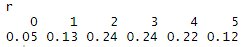
\includegraphics[scale=0.4]{probabilidad_condicionada.jpeg}\\
            \centering
            \caption{}\\
        Ahora vamos a utilizar la siguiente linea de código para calcular los vectores usando las simulaciones.\\
            
        \begin{lstlisting}
            # segunda forma 
            rango.dados2<- function(n){
              b1<-rep(0,n)
              for (i in 1:n) {
                  b1[i]= diff(range(sample(1:6,3,T)))
                }
              prob<-table(b1)/n
              return(b1)
            }
            rango.dados2(100)
        \end{lstlisting}
        El código debería ejecutado debería ejecutar lo siguiente:\\
        
            \centering
            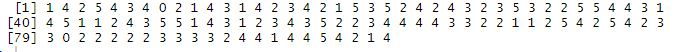
\includegraphics[scale=1]{probabilidad_condicionada1.JPG}
            \centering
            \caption{}
        \\
        Y por ultimo la ultima sentencia de código que vamos a utilizar va hacer de la siguiente manera \\
        \begin{lstlisting}
            # tercera forma
            rango.dados3<-function(n){
              b1<-c()
              b1<-replicate(n,sample(1:6,3,T))
              r1<-apply(b1,2,max)-apply(b1,2,min)
              prob<-table(r1)/n
              return(prob)
            }
            rango.dados3(100)
        \end{lstlisting}\\
        Ejecutado debe aparecer los vectores que se evalúan en las posiciones del 1 al 6.\\
        
        
            \centering
            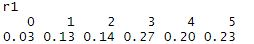
\includegraphics[scale=1]{probabilidad_condicionada2.JPG}\\
            \centering
            \caption{}
            
            
	\subsection{Bayes}
		\subsubsection{Teorema de Bayes                  }
		    El teorema de Bayes o regla de Bayes sea $B_1,..,B_n$ donde es una partición de de los posibles resultados, talque cada una de estas particiones la probabilidad sea distinta de cero (0)  Sea B un suceso cualquiera del que se conocen las probabilidades condicionales  $P(B|A)$. Entonces, la probabilidad $P(A|B)$ viene dada por la expresión:
		    \[
		    P(A/B)=\frac{P(B/A)P(A)}{P(B)}
		    \]
		    Donde cada probabilidad se define de la siguiente manera:
		    \begin{itemize}
		        \item P(A) son las probabilidades a priori
		        \item P$(B|A)$ es la probabilidad de $B$ en la hipótesis $A$
		        \item P$(A/B)$ son las probabilidades a posteriori. 
		    \end{itemize}
		    Ahora vamos a ejecutar un código para Bayes que funciona para cualquiera que sea el problema que se quiere ejecutar.
		    \begin{lstlisting}
		    print ("ingrese el porcentaje ")
                    porcentaje<-c(scan())
                    print ("ingrese la probabilidad ")
                    prob<-c(scan())
                    
                    funcionb<- function(porcentaje,prob){
                      suma <- 0.00
                      for(i in 1: length(porcentaje)){
                        suma<-suma+porcentaje[i]*prob[i]
                      
                      }
                      resta <- 0.00
                      probabilidad<-c()
                      for(i in 1:length(porcentaje)){
                        resta<-porcentaje[i]*prob[i]/suma
                        probabilidad<-c(probabilidad,resta)
                      }
                      return(probabilidad)
                    }
                    
                    print(funcionb(porcentaje,prob))

		    \end{lstlisting}\\
		Para probar que si funciona vamos a ejecutar un problema.
		
		Una empresa que fabrica celulares tiene dos maquinas A y B cada maquina fabrica el 60\% y 40\% de los celulares respectivamente y cada maquina tiene un 5\% y 10\% respectivamente de celulares defectuosos entonces ¿Cual es la probabilidad de que el celular haya sido fabricado por la maquina A sabiendo que es defectuoso?
		
		Usando el código simple vamos a digitar los porcentajes que van hacer \textbf{0.06} y\textbf{0.04} que son los porcentajes de fabricación de cada maquina, y después digitamos la probabilidad que es el defecto de cada maquina seran \textbf{0.05} y \textbf{0.10}
		nos va quedar como solución:\\
		    \centering
            
\includegraphics[scale=1]{Bayes.JPG}\\
            \centering
            \caption{}
            
            
	\subsection{Distribución binomial}
			Una distribución binomial es una distribución de probabilidad discreta que describe el número de éxitos al realizar en n experimentos independientes entre sí, acerca de una variable aleatoria.
			\\
			Se entiende como una serie de pruebas o
            ensayos en la que solo podemos tener 2
            resultados (sea éxito o fracaso), siendo el
            éxito nuestra variable aleatoria.
            \[P_{(x)}={n \choose r} p^{x}q^{n-x}\]
            \[P_{(x)}=\frac{n!}{(n-x)!x!}p^{x}q^{n-x}\]\\
            Donde:\\
            p= Probabilidad de éxito\\
            q= Probabilidad de fracaso\\
            x= Variable aleatoria\\
            n= Número de ensayos\\
            
            En R ya viene la función binomial y se puede usar de la siguiente manera \textbf{binom} pero no se usa así de simple se tiene que poner \textbf{dbinom} para usar la funcion binomial simple, probabilidad acumulada se usa \textbf{pbinom}, la inversa de la función de distribución, es decir, los percentiles \textbf{qbinom} y \textbf{rbinom} se usa para los valores binomiales generados.
            
            \textbf{Ejemplo}: Imaginemos que un 80\% de personas en el mundo han visto el partido  del final del último mundial de fútbol. Tras el evento, 4 amigos se reúnen a conversar. ¿Cuál es la probabilidad de que 3 de ellos hayan visto el partido?
            
            \begin{lstlisting}
                n <- 4
                p<- 0.8
                x <- 3
                dbinom(x,n,p)
            \end{lstlisting}
			nos va quedar como solución:\\
		    \centering
            
\includegraphics[scale=1]{binomial.JPG}\\
            \centering
            \caption{}
	\subsection{Distribución de Poisson}
			Esta distribución es una de las más importantes distribuciones de variable discreta, los experimentos que resultan en valores numéricos de una v.a $X$ y que representan el número de resultados durante un intervalo de tiempo dado o en una región específica frecuentemente se conocen como experimentos Poisson.
			\[
			P(x)=\frac{\mu^x \cdot e^{-\mu}}{x!}
			\]
			Veamos el siguiente ejemplo: Suponga que los accidentes de una calle siguen un proceso de Poisson con una taza de 2 accidentes por semana.\\
			\begin{itemize}
			    \item Hallar la probabilidad de que se comentan 5 accidentes durante la próxima semana.
			\end{itemize}\\
			Vamos a calcular mediante la función \textbf{pois} al igual que la función binomial tiene las mismas características,
			\textbf{dpois}, \textbf{ppois}, \textbf{qpois} y \textbf{rpois}
		    \textbf{dpois} es para la $x=X$ probabilidad acumulada se usa \textbf{ppois}, la inversa de la función de distribución, es decir, los percentiles \textbf{qpois} y \textbf{rpois} se usa para los valores binomiales generados.\\
		    Ahora para solucionar el ejemplo se usa el siguiente código:
		    \\
            Ejecutado el problema primero se halla lambda teniendo en cuenta que lambda se halla mediante, si 2 accidentes son por 1 (una) semana entonces por 5 accidentes en la siguiente semana entonces 
            \begin{center}
                $2\to 1 \\
                x\to 1
                $\\
                Entonces calcular la media y se encuentra que es dos, ese es el valor de lambda.
            \begin{lstlisting}
                x<-5
                lambda<-2
                dpois(x,lambda)
            \end{lstlisting}\\
            \end{center}
		    \centering
            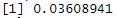
\includegraphics[scale=1]{poisson.JPG}\\
            \centering
            \caption{}
            
    \subsection{Distribución Z normal}
		En estadística y probabilidad se llama distribución normal, distribución de Gauss, distribución gaussiana o distribución de Laplace-Gauss, a una de las distribuciones de probabilidad de variable continua que con más frecuencia aparece en estadística y en la teoría de probabilidades.\\
		Una variable aleatoria continua, X, sigue una distribución normal de media $\mu$ y desviación típica $\sigma$, y se designa por N($\mu$,$\sigma$), si se cumplen las siguientes condiciones:
		\begin{itemize}
		    \item La variable puede tener valores desde ($-\infty,\infty$)
		    \item La función de densidad, es la expresión en términos de ecuación matemática de la curva de Gauss
		    \[
		        f(x)=\frac{1}{\sigma\sqrt{2\pi}}e^{-\frac{1}{2}(\frac{x-\mu}{\sigma})^2}
		    \]
		\end{itemize}
		Para estandarizar un valor de $X$:
		\[Z=\frac{x-\mu}{\sigma}\]
		Donde $\mu$ es la media y $\sigma$ es la distribución estándar.\\
		En R para hacer una distribución normal podemos usar la siguiente función \textbf{norm} al igual que las distribuciones de Poisson y binomial tiene:\\
		\textbf{dnorm}, \textbf{pnorm}, \textbf{qnorm} y \textbf{rnorm}.\\
		\textbf{dnorm} es para la $x=X$ probabilidad acumulada se usa \textbf{pnorm}, la inversa de la función de distribución, es decir, los percentiles \textbf{qnorm} y \textbf{rnorm} se usa para los valores binomiales generados.\\
		Vamos hacer el siguiente problema.\\
		 La temperatura durante septiembre está distribuida normalmente con media 18,7$\º$Cy desviación estándar 5$\º$C. Calcule la probabilidad de que la temperatura durante setiembre esté por debajo de 21$\º$C
		 \begin{lstlisting}
                x<-21
                media<-18.7
                desvia<-5
                pnorm(x,media,desvia)
            \end{lstlisting}\\
        Y la solución para el siguiente ejercicio es:\\
            \centering
            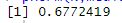
\includegraphics[scale=1]{normal.JPG}\\ \\
            \centering
            \caption{}
    \subsection{Intervalos de confianza}
        \subsubsection{Pruebas de hipótesis}
            Son procedimientos de decisión basado en datos que puedan producir una conclusión acerca de algún sistema científico.\\
            Una \textbf{hipótesis estadística} es una afirmación o conjetura acerca de una o más poblaciones.\\
            Tener en cuenta:
            \begin{itemize}
                \item Hipótesis nula  $H_0$: $\mu=\mu_0$; $\mu\leq\mu_0$; $\mu\geq\mu_0$
                \item Hipótesis Alternativa: $H_1:$ $\mu=\mu_1$; $\mu<\mu_1$; $\mu>\mu_1$; $\mu\neq\mu_1$
            \end{itemize}
            Para probar las hipótesis se tiene la prueba de normalidad de Kolmogorov-Smirnov, pruebas de variabilidad y pruebas de medias.
            \subsubsection{Prueba de normalidad}
            Los resultados de la prueba indican si usted debe rechazar o no puede rechazar la hipótesis nula de que los datos provienen de una población distribuida normalmente.
            \\ Vamos a usar la prueba de normalidad de Kolmogorov-Smirnov y de Shapiro Wilk
            \begin{itemize}
                \item \textbf{Prueba de normalidad de Kolmogorov-Smirnov}:\\
                Esta prueba compara la función de distribución acumulada empírica de los datos de la muestra con la distribución esperada si los datos fueran normales.
                Se va usar la el comando \textbf{lillie.test} hace el calculo de Kolmogorov-Smirnov mejorado para usar \textbf{lillie.test} tener en cuenta que toca instalar \textbf{nortest} y vamos a usar un ejemplo propio para eso, teniendo en cuenta que para Kolmogorov-Smirnov se usa para datos mayores a 50.
                \begin{lstlisting}
                set.seed(100)
                muestra<- rnorm(n=100,mean=170,sd=19)
                plot(density(muestra))
                library(nortest)
                lillie.test(muestra)$p.value
                
                \end{lstlisting}\\
                y su respuesta y gráfica serian las siguientes:\\
                \centering 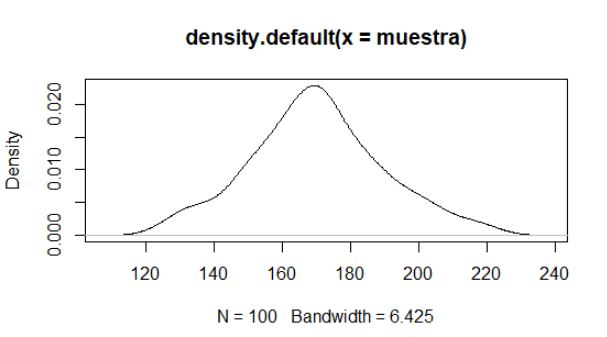
\includegraphics[scale=0.8]{ks_grafica1.jpeg}\\
                \centering
                \caption{}\\
                
                \centering
                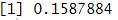
\includegraphics[scale=1]{ks1.JPG}\\ \\
                \centering
                \caption{respuesta Kolmogorov-Smirnov}
                
                \item \textbf{Prueba de normalidad Shapiro Wilk:}\\
                se usa para contrastar la normalidad de un conjunto de datos. Se plantea como hipótesis nula que una muestra $x_1,...,x_n$ proviene de una población normalmente distribuida\\
                \begin{lstlisting}
                    set.seed(50)
                    muestra<- rnorm(n=5,mean=10,sd=4)
                    plot(density(muestra))
                    library(nortest)
                    shapiro.test(muestra)$p.value
                    
                \end{lstlisting}\\
                \centering
                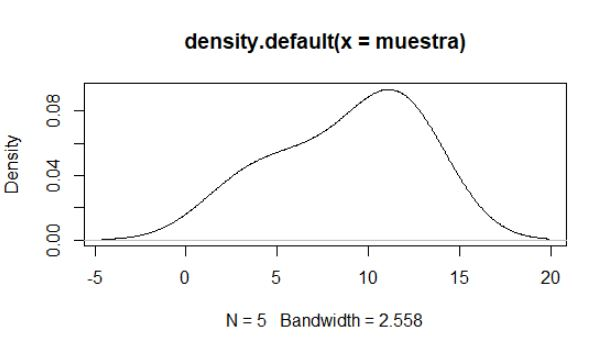
\includegraphics[scale=0.8]{ks_grafica.jpeg}\\
                \centering
                \caption{}\\
                
                \centering
                
\includegraphics[scale=1]{ks.JPG}\\ \\
                \centering
                \caption{respuesta Shapiro Wilk}
            \end{itemize}
        \subsection{Prueba de varianza}
        Pruebas de hipótesis para una varianza es un procedimiento para juzgar si una propiedad que se supone cumple una población estadística es compatible con lo observado en una muestra de dicha población en este caso la varianza, para ello formularemos dos Hipótesis (llamada "Hipótesis Nula") y (llamada "Hipótesis Alternativa"), con ellas realizaremos una o más pruebas, para tratar de encontrar cual se debe rechazar.
        \\ cuando se trabaja con varianza se utiliza $chi^2$ que es una prueba de hipótesis que compara la distribución observada de los datos con una distribución esperada de los datos., por lo tanto nos vamos a concentrar en $chi^2$.\\
        Entonces vamos a R para usar crear una hipótesis para usar $chi^2$ en R es simplemente usar \textbf{chisq.test}.\\
        \begin{lstlisting}
        fumar=matrix(c(51,43,22,59,56,45,48,78,95),ncol=3,byrow = TRUE)
        colnames(fumar) = c("mucho","poco","medio")
        rownames(fumar) = c("actual","pasado","nunca")
        fumar=as.table(fumar)
        fumar
        chisq.test(fumar)
        \end{lstlisting}\\
        En el código hemos creado nuestra hipótesis de fumadores donde creamos una tabla de contingencia, datos inventados.\\
            \centering
            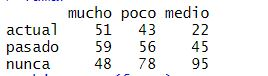
\includegraphics[scale=0.8]{chi.JPG}\\
            \centering
            \caption{}\\
        Y la respuesta de $chi^2$:\\
            \centering
            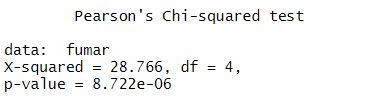
\includegraphics[scale=0.8]{chires.JPG}\\
            \centering
            \caption{}\\
    \subsection{Prueba de media}
    Se utiliza una prueba de una muestra para probar una afirmación con respecto a una media de una población única,en vez de estimar el valor de un parámetro, a veces se debe decidir si una afirmación relativa a un parámetro es verdadera o falsa.
    \\ En este caso Vamos a usar la prueba t que es muy buena que se utiliza cuando deseamos comparar dos medias (las cuentas se deben medir en una escala de intervalo o de cociente)\\
    Vamos A ejecutar un código en R de una prueba t student entonces para una prueba t student en E se necesita escribir el código con el siguiente código \textbf{t.test}.
        \begin{lstlisting}
        set.seed(10)
        x1 <- rnorm(100,10) 
        x2 <- rnorm(100,10.5) 
        test <- t.test(x1,x2)
        print(test)
        \end{lstlisting}\\
        Ejecutando el código.
            \centering
            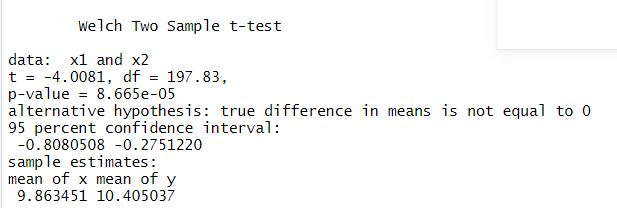
\includegraphics[scale=0.8]{t-s.JPG}\\
            \centering
            \caption{}\\
    Como el p-value es < 0.05 podemos afirmar que las muestras difieren en su media, es decir, las dos variables son diferentes con un gráfico de cajas se puede ayudar a interpretar este resultado,las medias se indican mediante un punto azul:\\   
    \begin{lstlisting}
        boxplot(x1,x2,names=c("X1","X2"))
        medias <- c(mean(x1),mean(x2))
        points(medias,pch=18,col="blue")
        \end{lstlisting}\\
            \centering
            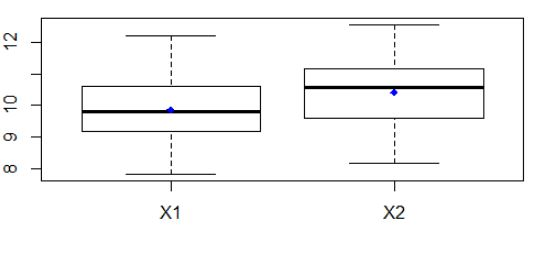
\includegraphics[scale=0.8]{grafica-t.JPG}\\
            \centering
            \caption{}\\
\newpage

%%%%%%%%%%%%%%%%%%%%%%%%%%%%%%%%%%%%%%%%%%%%%%%%%%%%%%%%%%%
\section{Spacing and Layout}
\vspace{10.5cm}
	\subsection{Geometry Package/Layout of the Document}
		The geometry package inside latex allows you to change the margins and layout of the document.
			\begin{docCommand}{newgeometry}{\brackets{left= mm, right= mm, top= mm, bottom= mm}} 
				This command allows you to change the margins and layout for that page and ones that come after it. This allows you to change the margins mid-document.
			\end{docCommand}
	\subsection{Centering}
		\subsubsection{Single-Line}
			If you have only one line to center, it’s easiest to use the plain TEX command \cs{centerline}; for example:
    		\begin{verbatim}
    	    \centerline{This line will be centered}.
    		\end{verbatim}
		\subsubsection{Multi-Line}
			If you have several lines to be centered horizontally, the center environment is convenient. Make sure when using this environment, to use the line break, see-    \ref{subsec:linebreaking}
			\begin{docEnvironment}{center}{}
			\end{docEnvironment}
	\subsection{Spacing and New Pages}
		\subsubsection{Inserting Horizontal and Vertical Space}
			\begin{docCommand}{vspace}{\brackets{distance}}
				This command allows you to insert a vertical space the distance that you specify in the brackets between items.
			\end{docCommand}
			\begin{docCommand}{hspace}{\brackets{distance}}
				This command allows you to insert a horizontal space a certain distance that you identify between items.
			\end{docCommand}
			\begin{docCommand}{vfill}{}
				This command inserts vertical white space spanning the current point on the page all the way down. Great if you want to include something on the bottom of the page but not quite a footer. 
			\end{docCommand}
		\subsubsection{Page and Line Breaks}\label{subsec:linebreaking}
			\begin{docCommand}{newpage}{}
				This command forces a page break at that point in the text. 
			\end{docCommand}
		The following command is how to terminate a line/force a line to break:
			\begin{verbatim} \\ \end{verbatim}
		\subsubsection{Indenting}
			\begin{docCommand}{noindent}{}
				This commands allows you to prevent text from being indented.
			\end{docCommand}
			\begin{docCommand}{indent}{}
				Similarly, this command allows you to force the text to indent.
			\end{docCommand}
		\subsubsection{Line Spacing}
			If you want to use larger inter-line spacing in a document, change its value by putting the
			\begin{verbatim}
				\linespread{factor}
			\end{verbatim}
			command into the preamble of your document. Use \cs{linespread\brackets{1.3}} for “one and a half” line spacing, and \cs{linespread\brackets{1.6}} for “double” line-spacing. Normally the lines are not spread, so the default line spread factor is 1.
			Note that the effect of the \cs{linespread} command is rather drastic.
		\subsubsection{Math Spacing}
			\begin{docCommand}{quad}{}
				Creates a horizontal space equal to the current font size (= 18 mu)
			\end{docCommand}
			\begin{docCommand}{;}{}
				5/18 of \cs{quad} (= 3 mu)
			\end{docCommand}
			\begin{docCommand}{:}{}
				4/18 of \cs{quad} (= 3 mu)
			\end{docCommand}
			\begin{docCommand}{,}{}
				3/18 of \cs{quad} (= 3 mu)
			\end{docCommand}
	\subsection{Margin Notes}
	The package labeled margin notes contained within the folder holding this file allows for the user to write text in the margins.
		\begin{docCommand}{marginnote}{\brackets{\sl{text}}[distance offset]}
				This command inserts a note in the margin on the right hand side. When using the margin note, remember to use the line break command: % - \\ 
				Also remember to specify and adjust the vertical offset of the margin note.
		\end{docCommand}
		\begin{docCommand}{reversemarginpar}{\cs{marginnote}\brackets{\sl{text}}}
				This command with the reverse marginpar creates a note in the margin on the left hand side of the document.\\
				Insert the text for the marginnote in place of \marg{text}.
		\end{docCommand}
		\subsubsection{Adjusting the Width of a Margin Note}
			\begin{docCommand}{marginparwidth}{}
					This command allows you to specify the width you would like the margin to be. Input this in the geometry command in your preamble or typing \cs{newgeometry{marginparwidth=distance}}
			\end{docCommand}
			\begin{docCommand}{marginparsep}{}
					This allows you to specify the distance between the margin note and the main text. Input this in the geometry command in your preamble or typing \cs{newgeometry{marginparsep=distance}}
			\end{docCommand}
\newpage
%%%%%%%%%%%%%%%%%%%%%%%%%%%%%%%%%%%%%%%%%%%%%%%%%%%%%%%%%%%
\section{Tests/Exams}	
\vspace{10.5cm}	
	\subsection{Math Environments}\label{subsec:mathenvironments}
		\begin{docEnvironment}{displaymath}{}
			Environment for equations that are on their own line and centered. In the displaymath environment no equation number is added to the math text. One way to get an equation number is to use the equation environment
		\end{docEnvironment}
		\begin{docEnvironment}{equation}{}
			Similar to the displaymath environment, such adds a equation number on the right side of the document.
		\end{docEnvironment}	
		\begin{docEnvironment}{math}{}
			For formulas that appear right in the text. 
		\end{docEnvironment}
	\subsection{Structuring}
		\begin{docCommand}{leqno}{}
			Equation numbers in displayed formulas will appear on the left instead of the normal right side.
		\end{docCommand}
		\begin{docCommand}{fleqn}{}
			Displayed formulas will be set flush left instead of centered.
		\end{docCommand}
	\subsection{Writing Exams}\label{subsec:writingexams}
		\subsubsection{Questions}
			\begin{docEnvironment}{questions}{}\label{questionenv}
				To create questions, use this questions environment. 
			\end{docEnvironment}
			\begin{docCommand}{question}{}
				Once you have created the question environment, you can begin questions using the \cs{question} command.
			\end{docCommand}
			\begin{docCommand}{vspace1}{\brackets{\cs{stretch}\brackets{1}}}
			    \textbf{Replace \cs{vspace1} with \cs{vspace}}\\
				This command allows you to evenly space questions along the page.
			\end{docCommand}
		\subsubsection{Choices}
			\begin{docEnvironment}{choices}{}
				To create choices for a questions, use this environment. 
			\end{docEnvironment}
			\begin{docCommand}{choice}{}
				This command allows you to create choices inside of the choices environment.
			\end{docCommand}
	\subsubsection{Displaying Solutions}
		The exam document class defines several environments for solutions, the contents of which will be printed only if you use the document class option answers as in the:\\ \begin{verbatim} 
		\documentclass[answers]{exam}
		\end{verbatim}
		which you can find by going to the examMC .tex file within the folder originally containing this document and adding [answers] at the top of the preamble at the document class or give the command \cs{printanswers}.\\ \vspace{1.5mm}
		Each of the environments for multiple choice questions
		designate one or more of the choices as correct choices, and to have the correct choices printed with emphasis \emph{only}when solutions are being printed.\vspace{1.5mm}\\ 
		The command to define a correct choice is \cs{CorrectChoice}, which is used in place of the command \cs{choice}. (To avoid confusion, \cs{correctchoice} is defined to be a synonym
		for \cs{CorrectChoice}) When solutions are not being printed, \cs{CorrectChoice} is equivalent to \cs{choice}. When solutions are being printed, though, any choices that were created with
		\cs{CorrectChoice} (rather than with \cs{choice}) will be printed in bold.
			\begin{docCommand}{correctchoice}{}
			\end{docCommand}
		\subsubsection{Source Code - Questions}
			\begin{verbatim}
			\begin{questions}
				\question \quad
				{If $\textit{f}(x) = \frac{1}{4}x^4+x^3$ What is $\frac{d}{dx}$?}
					\vspace{2mm}
					\begin{choices}
						\choice 5x
						\correctchoice $20x^3$+$3x^2$
						\choice $x^3$+$3x^2$
						\choice 2x
						\choice $20x^2$
					\end{choices}
					\vspace{\stretch{1}}
			\end{verbatim}
		\subsubsection{Source Code - Questions with Image on the side}
			\begin{verbatim}		
			\question \quad 
			\begin{minipage}[t]{0.65\linewidth}
			{$\int{(3x + 1)^5}$\textit{dx}} =
			\vspace{2mm}
			\begin{choices}
			\correctchoice \large{$\frac{(3x + 1)^6}{18} + C $}
			\choice \large{$\frac{(3x + 1)^6}{6}$ + C}
			\choice \large{$\frac{(\frac{3x}{2} + 1)^6}{2}$ + C}
			\choice \large{$\frac{(3x + 1)^6}{2}$ + C}
			\choice \large{$(\frac{3x}{2} + x)^5$ + C} 
			\end{choices}
			\end{minipage}\hfill%
			\begin{adjustbox}{minipage={0.30\linewidth},valign=t}
			\includegraphics[width=\linewidth]{example-image-a}
			\end{adjustbox}
			\vspace{\stretch{1}}
			\end{verbatim}
	\subsection{Math Commands}
		\begin{docCommand}{boxed}{}
			Inserts a box around an equation.
		\end{docCommand}
\newpage
%%%%%%%%%%%%%%%%%%%%%%%%%%%%%%%%%%%%%%%%%%%%%%%%%%%%%%%%%%%
\section{List of Already Defined Environments and Macros}	
\vspace{10.5cm}
The following subsections are lists and examples of pre-defined macros or commands. Creating a macro in latex is effectively similar to creating a shortcut. Macros allow for a cleaner, more efficient process of writing the code for your document. \\
Macros are great for repetitive elements and texts that you carry across several documents.
	\subsection{Main Box Environments}
		\subsubsection{Theorems}
			\begin{docEnvironment}{theo}{}
				This environment \cs{begin\brackets{Theo}} inserts a new yellow theorem box with a black frame into the document. 
			\end{docEnvironment}
		\subsubsection{Boxes for Definitions}
			\begin{docEnvironment}{definition}{}
				This environment \cs{begin\brackets{definition}} inserts a regular definition into the document. 
			\end{docEnvironment}
		\subsubsection{Boxes for Examples}
			\begin{docEnvironment}{example}{\brackets{\sl{title}}}
				This environment \cs{begin\brackets{example}} creates a regular example box. \\
				After inserting the question for the specified example, make sure to use the command \cs{tcbline} or \cs{tcblower}. This command creates a dashed line within the example box or any pre-created box and allows for you to created a specified space for the students to fill in the solution. 
			\end{docEnvironment}
			\begin{docEnvironment}{longexample}{\brackets{\sl{title}}}
				Environment for creating examples inside lessons whose text is quite lengthy or the example requires a good amount of work or drawing. \\
				If one wants to extend the box of the height further that the default value, go to the lesson.tex file inside of the lessons folder. Once inside of the lesson.tex file, go down to about line 136, inside the examstyle./style, and change the height from 9.5cm to your preferred value. 
			\end{docEnvironment}
		\subsubsection{Boxes for Discussions}
			\begin{docEnvironment}{discussion}{\brackets{\sl{title}}}
				This environment inserts a box similar to the example box just instead labeled discussion. \\ 
				Similar to the example box as well, after inserting the question or text, make sure to use the command \cs{tcbline}. This command will create a dashed line within the box and allows for you to created a specified space for the students to fill in the solution or drawing etc. preferred value. 
			\end{docEnvironment}
		\subsubsection{Boxes for Visualizations}
			\begin{docEnvironment}{visualization}{\brackets{\sl{title}}}
				This environment inserts a box similar to the example and discussion boxes just instead for visualizations. 
			\end{docEnvironment}
	\subsection{Extra Box Environment}
		\begin{docEnvironment}{DashedDefinition}{}
			This command offers another option for a definition box just with a dashed frame.
		\end{docEnvironment}
\vspace{2mm}		
\newgeometry{
	left=14mm, 
	right=14mm, 
	top=9mm, 
	bottom=13mm}
%%%%%%%%%%%%%%%%%%%%%%%%%%%%%%%%%%%
% ------- Code & Examples ------- %
%%%%%%%%%%%%%%%%%%%%%%%%%%%%%%%%%%%
\begin{disexam}
\begin{DashedDefinition}{}
[A partial derivative of a function of several variables is its derivative with respect to one of those variables, with the others held constant. Partial derivatives are used in vector calculus and differential geometry.
\end{DashedDefinition}
\end{disexam}
\vspace*{0.75\baselineskip}
%===============================
\begin{disexam}
\vspace{1mm}
\begin{visualization}[\quad \large Angular Momentum \hspace{3mm}]
Discuss an alternate way of using the conservation of angular momentum for satellite orbits and any other point masses moving in a circle.
\tcbline
\end{visualization}
\vspace{1mm}
\end{disexam}
\vspace*{0.75\baselineskip}
%===============================
\begin{disexam}
\begin{example2}
\vspace{1mm}
A partial derivative of a function of several variables is its derivative with respect to one of those variables, with the others held constant. Partial derivatives are used in vector calculus and differential geometry.
\tcbline
\end{example2}
\end{disexam}
%===============================
	\vspace*{1\baselineskip}
\begin{disexam}
\begin{example}[\quad \large Rotational Motion]
Now assume the small pulley has rotational inertia.
\begin{enumerate}
\item Will your answers be different? Why?
\item How does the angular velocity of the rotating apparatus and the linear velocity of the falling mass compare to the previous case?
\item How does the torque exerted by the string on the rotating apparatus change the angular momentum of the apparatus?
\end{enumerate}
\tcbline
\vspace{1mm}
\solution
\end{example}
\end{disexam}
%===============================
\begin{disexam}
\begin{longexample}[\quad \large Rotational Motion]
A block of mass $4m$ is attached to a light string and passes over a pulley with negligible rotational inertia and is wrapped around a vertical pole of radius $r$.  The block is then released from rest, causing the string to unwind and the vertical pole it is wrapped around to rotate.  On top of the vertical pole lies a horizontal rod of length $2L$ with block2s of mass $m$ attached to both ends.  The rotational inertia of this apparatus is $2mL^2$.
\begin{enumerate}
\item What is the tension in the string in terms of the acceleration of the falling block?
\item What is the torque exerted on the rotating pole by the string in terms of the acceleration of the falling block?
\item When the large block has fallen a distance $D$, what is the instantaneous rotational kinetic energy of the apparatus?
\end{enumerate}
\tcblower
\vspace{1mm}
\solution
\end{longexample}
\end{disexam}
%===============================
\newgeometry{
	left=29mm, 
	right=29mm, 
	top=20mm, 
	bottom=15mm}
%===============================
\vspace{1.5mm}
	\subsection{Extra Box Commands}
		\begin{docCommand}{tcbline or tcblower}{}
				Creates a dashed line within the box. Useful for creating a specified portion for students to write their answer down.
		\end{docCommand}
		\begin{docCommand}{solution}{}
				Inserts the word solution in red font.
		\end{docCommand}
	\subsection{Commands (Macros)}
		\begin{docCommand}{contactinfo}{}
				Allows for a quicker way to input contact information through several documents.\\ 
				To insert contact information, put the following in your preamble:\\ \cs{newcommand}\brackets{\cs{contactinfo}}\brackets{Insert info here.}
		\end{docCommand}
		\begin{docCommand}{fillin}{}
			Allows for a quicker way to input a line for students to fill in the notes.
		\end{docCommand}
	\subsection{How to Define New Commands (Macros) and Colors}
		\begin{docCommand}{newcommand}{\brackets{\cs{name}}\brackets{\cs{action}}}
			The command \cs{newcommand} allows the user to effectively use a shortcut for a given action. Allows for a cleaner, more organized code. When creating a new command, make sure to put it in the preamble of you document.  
		\end{docCommand}
		\begin{docCommand}{definecolor}{\brackets{name for color}\brackets{rgb}}
			The \cs{definecolor} command allows for the user to define new colors to be used in the document. For the rgb values of different colors, go to latexcolor.com.
		\end{docCommand}
\newpage
%%%%%%%%%%%%%%%%%%%%%%%%%%%%%%%%%%%%%%%%%%%%%%%%%%%%%%%%%%%
\section{Inserting Graphics}
\vspace{10.5cm}
	Inserting graphics in your document requires the  \textbf{graphicx package}, which you can find in the folder that accompanied this guide.
	\subsection{Easiest Way to Insert Images}
	The easiest, most straightforward way I have found so far to insert images into your LaTeX document is through TeX Studios include graphics feature. This features allows you to bypass having to constantly type and communicate with your computer where the folder containing your images is located. This really comes in handy once one has created several latex documents across several folders. If you decide to insert images through this method, as I presume most of those reading this will, \textbf{make sure to remove the graphics path command from the preamble of the templates in the folder containing this pdf.}
\vspace{4mm}\\
	So to insert an image into your \LaTeX\ file, go to the taskbar located at the top of your screen and click the menu labeled \textbf{LaTeX}. Inside the LaTeX dropdown, go down to \textbf{Input/Include Files} and then \textbf{includegraphics}. Once there, find where you put the image you wanted to insert into your document and then press ok.
	\subsection{Graphics Path}
	Most of the time, it will easier to insert images into a file using the method we mentioned in the previous subsection. However, the following allows for a cleaner, more organized, but a little more complicated at times possibly more advanced way to insert images into your \LaTeX\ file.
		\begin{docCommand}{graphicspath}{\brackets{path}}
			This command prevents you from having to tell the computer where the image is stored each time you wanted to insert an image.\\
			The easiest way to set up the graphicspath is to create a folder where you store all the images you want to use and label it \textbf{images}. You put this folder in the same area where you write your files. Then you input the following at the beginning of your document: 
			\begin{verbatim}
				\graphicspath{{./images/}}
			\end{verbatim}
		\end{docCommand}
	\subsection{Inserting Images}
		Once you have set up the graphics path from above, you insert pictures by using the following command:
		\begin{docCommand}{includegraphics}{\brackets{\sl{file-name}}}
			This command allows you to actually insert the image in the document. To alter the position and size of the image, see~\url{https://www.overleaf.com/learn/latex/Inserting_Images}.\\
		\end{docCommand} \vspace{1mm}
		To change the scale of file, use the following
		\begin{verbatim}
			\includegraphics[scale= ]{image file name}
		\end{verbatim}
	\subsection{Image Additions}
		\begin{docCommand}{caption}{\brackets{\sl{text}}}
			Allows you to add a caption to an image.
		\end{docCommand}
		\begin{docEnvironment}{wrapfigure}{}
			Allows you to wrap an image inside text. For more on this, see the wrapfigure.pdf inside the wrapfigure folder.
		\end{docEnvironment}
	\subsection{Positioning an Image}
		To alter an images position: see \url{https://www.overleaf.com/learn/latex/Inserting_Images}
\newpage
\newgeometry{
	left=20mm, 
	right=20mm, 
	top=20mm, 
	bottom=20mm}
%%%%%%%%%%%%%%%%%%%%%%%%%%%%%%%%%%%%%%%%%%%%%%%%%%%%%%%%%%%
\section{Font Styles}
\vspace{10.5cm}
	\subsection{Font Types}
\[\begin{array}{ccc}
\cs{textit\brackets{...}} & \textit{italic} & \textup{Italic shape, used mostly for emphasis.}\\
\cs{textsl\brackets{...}} & \textsl{slanted} & \textup{Slanted shape, a bit different from italic.}\\
\cs{textsc\brackets{...}} & \textsc{Small Caps} & \textup{Small caps shape, use sparingly.}\\
\cs{textup\brackets{...}} & \textup{upright} & \textup{Upright shape, usually the default.}\\
\cs{textbf\brackets{...}} & \textbf{boldface} & \textup{Boldface series, often used for headings.}\\
\cs{textmd\brackets{...}} & \textmd{medium} & \textup{Medium series, usually the default.}\\
\cs{textrm\brackets{...}} & \textrm{roman} & \textup{Roman family, usually the default.}\\
\cs{textsf\brackets{...}} & \textsf{sans serif} & \textup{Sans Serif family, used for posters, etc.}\\
\cs{texttt\brackets{...}} & \texttt{typewriter} & \textup{Typewriter family, fixed-pitch characters.}\\
\cs{emph\brackets{...}} & \emph{emphasized} & \textup{Use for emphasis, usually changes to italic.}\\		
\end{array}\]
\newpage
\newgeometry{
	left=32mm, right=18mm, top=20mm, bottom=18mm,
	marginparwidth=28mm, marginparsep=4mm}
%%%%%%%%%%%%%%%%%%%%%%%%%%%%%%%%%%%%%%%%%%%%%%%%%%%%%%%%%%%
\section{Referencing and Documentation}
\vspace{10.5cm}
	\subsection{References/Hyperlinks and Formatting}
		\begin{docCommand}{label}{\brackets{\sl{link}}}
			In order to refer to make a cross-reference within a document, you first must label the text/section that you want to refer to.
		\end{docCommand}
		\begin{verbatim}
	            \subsection{Math Tests/Exams and Math Symbols/Functions}\label{mathexams}
		\end{verbatim}
		\begin{docCommand}{ref}{\brackets{\sl{label-name}}}
			This command allows you to make a cross-reference to another part of your document. 
		\end{docCommand}
		\begin{docCommand}{href}{\brackets{\sl{label-name}}}
			This command is used when the user wants to insert a link that is able to clicked on into a document but want's there to be a placeholder to cover the hyperlink. An example is below. 
		\end{docCommand}
\begin{disexam}
\href{mailto:armindubert19@gmail.com}{basis independent mclean}
\end{disexam}
		\begin{docCommand}{fullref}{\brackets{\sl{label-name}}}
			This command allows you to make a cross-reference to another part of your document. The \cs{fullref} includes both the section and page number that you are referring to as opposed to the command \cs{ref} that only refers to the section.
		\end{docCommand}
		\begin{docCommand}{url}{\brackets{\sl{link}}}
			This command allows you to insert a link into your document that's able to be clicked on in the pdf you create.
		\end{docCommand}
		\begin{docCommand}{hypersetup}{\brackets{colorlinks,linkcolor={red!50!black},citecolor={blue!50!black}, urlcolor={blue!80!black}}}
			This following command makes the links you include in your code/file more appealing by removing the box around the links as well as color coding the different links. This command should be inserted in the preamble of your document.
		\end{docCommand}
	\subsection{Documentation}
	Documentation and Listings are commands and ways of showing source code side by side with the behavior of the command.\\
	To use documentation in latex, make sure to input \cs{tcbuselibrary}\brackets{listings}.
		\begin{docCommand}{cs}{}
			Allows you to typeset a command without having the command actually played out.
		\end{docCommand}
		\begin{disexam}
\cs{marg}
		\end{disexam}
		\begin{docCommand}{brackets}{}
			Allows you to put brackets around text that will appear in the document.
		\end{docCommand}
		\begin{disexam}
\cs{brackets}
		\end{disexam}
		\begin{docEnvironment}{docCommand}{}
			Allows you to identify a command and define what it does, similar to all of the lines with a yellow background in this pdf.
		\end{docEnvironment}
		For more on documentation, see tcolorbox.pdf
	\subsection{Verbatim}
		To reproduce new lines and spaces exactly as they are in your input file, use the verbatim environment. The verbatim environment prints its text in typewriter-style type and sets it off from the rest of the document with blank lines before and after.
		\begin{docEnvironment}{verbatim}{}
			Allows you to identify a command and define what it does, similar to all of the lines with a yellow background in this pdf.
		\end{docEnvironment}
\newpage
%%%%%%%%%%%%%%%%%%%%%%%%%%%%%%%%%%%%%%%
	\subsection{Source Code for the Documentation Style used in this PDF}
	The following source code is for the customized environment for the documentation boxes in this pdf. 
		\begin{verbatim}
		\newtcblisting[auto counter,number within=section]{disexam}{
		skin=bicolor,
		colback=white!30!beaublue,
		colbacklower=white,
		colframe=black,
		before skip=\medskipamount,
		after skip=\medskipamount,
		fontlower=\footnotesize,
		listing options={style=tcblatex,texcsstyle=*\color{red!70!black}}}
		\end{verbatim}
\newpage
%%%%%%%%%%%%%%%%%%%%%%%%%%%%%%%%%%%%%%%%%%%%%%%%%%%%%%%%%%%
\section{Common Symbols and Functions}
\vspace{10.5cm}
When it comes to typing symbols, \LaTeX\ has a library that makes it easier to insert symbols into a\\ document. While it does not have all of them, it does provide a good handful them.\\
To access the library, go to the bottom left corner of \LaTeX\ where one will see the following boxes:\\	
Once you have found this, click the button on the left until you have the white side bar on the left that contains the structure along with some other features. (Note, when you first open \LaTeX\ this sidebar is usually already open. However, I want to make sure users are aware what to do in the case they accidentally close the sidebar).\\
Once the sidebar is opened, go to the third one down, on the furthest left hand side, which should look something like this:\\
Once you have clicked on this, feel free to explore some of the symbols inside the library along with the other button features on the sidebar.\\ 
If there are some symbols that you regularly and are not contained in that library, check the following symbols in this section or see: \url{https://www.caam.rice.edu/~heinken/latex/symbols.pdf}
	\subsection{Functions}
	For a comprehensive and detailed guide for Math Functions, see:\\ \url{https://artofproblemsolving.com/wiki/index.php/LaTeX:Commands}
		\begin{docCommand}{sqrt}{\brackets{abd}}
			$\sqrt{abd}$
		\end{docCommand}
		\begin{docCommand}{sqrt1}{[n]\brackets{abd}}
		    \textbf{Replace \cs{sqrt1} with \cs{sqrt}}\\
			$\sqrt[n]{abd}$
		\end{docCommand}
	\subsection{Limits, Integrals, Sums, and Fractions}
		For a more complete instruction on how to write limits, integrals, and sums in latex, see:\\
		\url{https://artofproblemsolving.com/wiki/index.php/LaTeX:Commands}
		\begin{docCommand}{int}{}
			\begin{verbatim}
				$\int_{lower}^{upper}$
			\end{verbatim}
			This is the command for creating integrals. Make sure when using to put it in a Math Environment, see \fullref{subsec:mathenvironments} or put dollar signs on both sides of the integral.
		\end{docCommand}
		\begin{docCommand}{dfrac}{\brackets{\sl{abc}}\brackets{\sl{xyz}}}{}
			\begin{verbatim}
				$\dfrac{abc}{xyz}$
			\end{verbatim}
			$\dfrac{abc}{xyz}$
			This is the command for creating Fractions. Make sure when using to put it in a Math Environment, see \fullref{subsec:mathenvironments} or put dollar signs on both sides of the fraction.
		\end{docCommand}
		\begin{docCommand}{sum}{}
			\begin{verbatim}
				$\sum_{lower}^{upper}$
			\end{verbatim}
			This is the command for creating Summations. Make sure when using to put it in a Math Environment, see \fullref{subsec:mathenvironments} or put dollar signs on both sides of the Summation.
		\end{docCommand}	
		\begin{docCommand}{lim}{}
			\begin{verbatim}
			$$\lim_{x\to\infty} f(x)$$
			\end{verbatim}
			$$\lim_{x\to\infty} f(x)$$
			This is the command for creating Limits. Make sure when using to put it in a Math Environment, see \fullref{subsec:mathenvironments} or put two dollar signs on both sides of the limit.
		\end{docCommand}	
	\subsubsection{Symbols}
		\begin{docCommand}{Delta}{}
			$\Delta$
		\end{docCommand}
		\begin{docCommand}{pi}{}
			$\pi$
		\end{docCommand}	
		\begin{docCommand}{theta}{}
			$\theta$
		\end{docCommand}
		\begin{docCommand}{leq}{}
			$\leq$
		\end{docCommand}
		\begin{docCommand}{geq}{}
			$\geq$
		\end{docCommand}
		\begin{docCommand}{leqq}{}
			
		\end{docCommand}	
		\begin{docCommand}{neq}{}
			$\neq$
		\end{docCommand}
		\begin{docCommand}{approx}{}
			$\approx$
		\end{docCommand}
\newpage
%%%%%%%%%%%%%%%%%%%%%%%%%%%%%%%%%%%%%%%%%%%%%%%%%%%%%%%%%%%
\section{Bibliography}
\vspace{10.5cm}
The following environment and command creates a clean and organized bibliography.
	\begin{docEnvironment}{thebibliography}{\brackets{\emph{numberofsources}}}
			The following environment is needed to create the bibliography.
	\end{docEnvironment}
	\begin{docCommand}{bibitem}{}
			The following command creates each source.
	\end{docCommand}
\newgeometry{
	left=20mm, right=20mm, top=25mm, bottom=25mm}
\subsection{Bibliography Source Code}
Spacing is just used to help show the different commands and environments. Do not feel obligated to\\
include the spacing exactly how it is.\\
\hrule
	\vspace{4mm}
\begin{verbatim}
\begin{thebibliography}{5 % - Number of Sources You are Citing}

\bibitem{financialbrand}Jim, M. (2018). \emph{10 Technologies That 
Will Disrupt Financial Services In The Next 5 Years.}\\
Retrieved from:\\
\url{https://thefinancialbrand.com/77228/technology-trends-disrupting
\\-financial-services-banking-future/}

\bibitem{Forbes} Alan, M. (2018). \emph{How Banks Should Navigate
as Their North Star Shifts.}\\
Retrieved from:\\ 
\url{https://www.forbes.com/sites/alanmcintyre/2018/10/18/how-banks-should-
navigate-through-digital-disruption-as-their-north-star\\-shifts/#39c502223ee7}

\bibitem{americanbanker} Penny, C., Will, H., Suleman, D. (2019). \emph{10 way 
technology will change banking in 2019.}\\
Retrieved from:\\ 
\url{https://www.americanbanker.com/list/10-ways-technology-will-change
-banking\\-in-2019}

\bibitem{Robert Wright} Wright, Robert. (2008). \emph{Origins of Commercial Banking
in the United States, 1781-1830. EH.Net Encyclopedia.}\\
Retrieved from:\\							
\url{http://eh.net/encyclopedia/origins-of-commercial-banking-in-the
\\-united-states-1781-1830/}

\bibitem{The Economist} \emph{Tech’s raid on the banks.} (2019). 
The Economist, 431(9141), 9.

\end{thebibliography}
\end{verbatim}
\newpage
\newgeometry{
	left=29mm, 
	right=29mm, 
	top=20mm, 
	bottom=20mm}
%%%%%%%%%%%%%%%%%%%%%%%%%%%%%%%%%%%%%%%%%%%%%%%%%%%%%%%%%%%
\section{Miscellaneous}
\vspace{10.5cm}
	\subsection{Rule}
		\begin{docCommand}{rule}{\brackets{\sl{length}}\brackets{thickness}}
				This command inserts a horizontal line with the designated width and thickness.
		\end{docCommand}
		\begin{docCommand}{hrulefill}{}
				Inserts a horizontal line that spans the entire width of the page.
		\end{docCommand}
		\begin{docCommand}{vrule}{\brackets{\sl{height}}\brackets{\sl{thickness}}}
				This command inserts a vertical line with the designated width and thickness.
		\end{docCommand}
\newpage
%%%%%%%%%%%%%%%%%%%%%%%%%%%%%%%%%%%%%%%%%%%%%%%%%%%%%%%%%%
\section{Some Common Errors}
\vspace{10.5cm}
	\begin{itemize}
		\item A command was misspelled and LATEX doesn’t recognize it.
		\item You have a special character \begin{verbatim}(e.g., &, $, #, %) in the text. Enter these as \&, \$, \# or \%.\end{verbatim}
		\item \begin{verbatim} Whatever you \begin{...}, you must \end{...}. This includes braces: { ... }.\end{verbatim}
		\item A command was not given all its arguments and is trying to use the rest of the file for an argument.
	\end{itemize}
\newpage
%%%%%%%%%%%%%%%%%%%%%%%%%%%%%%%%%%%%%%%%%%%%%%%%%%%%%%%%%%%
\section{Further Reading}\label{sec:resources}
\vspace{10.5cm}
	\subsection{Websites and Tutorials}
		If you are interested in understanding how Latex really works, I highly encourage reading the following package pdfs/websites/tutorials:\\
		If you are looking for a solution for a problem you have encountered and can not find it within these files, see the templates created in the folder that orignially contained this pdf file or contact me at: \url{armindubert19@gmail.com}
	\subsection{Introduction/Commands/and Overall Good References}
		\subsubsection{Writing First Document}
			\begin{itemize}
				\item \url{http://ctan.org/pkg/first-latex-doc}
					\begin{absquote}
						Writing your first document, with a bit of both text and math.
					\end{absquote}
			\end{itemize}
		\subsubsection{Brief Introduction/List of Commands}
			\begin{itemize}
				\item \url{https://www.scss.tcd.ie/~dwoods/1617/CS1LL2/HT/wk1/commands.pdf}
						\begin{absquote}
							This online article is an extremely brief reference guide for some Latex Commands.
						\end{absquote}
				\item \url{https://www.bu.edu/math/files/2013/08/LongTeX1.pdf}
						\begin{absquote}
							List of several useful commands.
						\end{absquote}
			\end{itemize}
		\subsubsection{In-Depth LaTeX Guide}
			\begin{itemize}
				\item \url{https://tobi.oetiker.ch/lshort/lshort.pdf}
						\begin{absquote}
							This online article is a semi-lengthy but thorough introduction to \LaTeX\. Great for people who are just starting.
						\end{absquote}
				\item \url{https://www2.mps.mpg.de/homes/daly/GTL/gtl_20030512.pdf}
						\begin{absquote}
							Another extensive guide that does a good job teaching the basics as well as go a little more in depth.
						\end{absquote}
				\item \url{http://www.rpi.edu/dept/arc/docs/latex/latex-intro.pdf}
						\begin{absquote}
							Another extensive guide that does a good job teaching the basics as well as going a little more in depth in some areas. 
						\end{absquote}
			\end{itemize}
	\subsection{Boxes}
		While this source is long, it provides great insight that leads to a greater understanding of the entire \LaTeX \, system. So if you are eager to dig deep into the latex language, the following source is a great place to start.
		\begin{itemize}
			\item tcolorbox.pdf
				\begin{absquote}
					This source is contained in the folder along with this file. This source is the longest source out of all the sources but is packed with information about all the great things you can do with boxes, such as the ones seen in this guide.	
				\end{absquote}
		\end{itemize}
	\subsection{Typesetting Math Documents}\label{sec:exams}
		\subsubsection{Creating Math Documents}
			\begin{itemize}
				\item \url{http://www-math.mit.edu/~psh/exam/examdoc.pdf}
					\begin{absquote}
						Extensive guide on how to write exams.  
					\end{absquote}
				\item mathexam.pdf
					\begin{absquote}
						You will find this source in the mathexam folder after having downloaded the mathexam.zip file onto your computer. This is a great source if you want to learn an alternate way to creating math test/exam using latex.
					\end{absquote}
			\end{itemize}
		\subsubsection{Symbols}
			\begin{itemize}
				\item \url{https://www.caam.rice.edu/~heinken/latex/symbols.pdf}
					\begin{absquote}
						List of Mathematical Symbols.
					\end{absquote}
				\item \url{https://www.bu.edu/math/files/2013/08/LongTeX1.pdf}
					\begin{absquote}
						An additional list of  Symbols.
					\end{absquote}
			\end{itemize}
		\subsubsection{Typing Math Functions/Equations}
			\begin{itemize}
				\item \url{https://www.overleaf.com/learn/latex/Integrals,_sums_and_limits}
					\begin{absquote}
						Goes over typesetting Integrals, Summations, and Limits.
					\end{absquote}
				\item \url{https://www.overleaf.com/learn/latex/Subscripts_and_superscripts}
					\begin{absquote}
						Goes over typesetting subscripts and superscripts
					\end{absquote}
				\item \url{https://www.overleaf.com/learn/latex/Fractions_and_Binomials}
					\begin{absquote}
						Goes over typesetting fractions and binomials.
					\end{absquote}
			\end{itemize}
	\subsection{Graphics}
		\subsubsection{Images}
			\begin{itemize}
				\item graphicx.pdf
					\begin{absquote}
						This source provides a great introduction for people interested in exploring the intricacies behind inserting images into a document.
					\end{absquote}
				\item \url{https://www.overleaf.com/learn/latex/Inserting_Images}
					\begin{absquote}
						Goes over some of the specifics behind setting up the \cs{graphicspath} and inserts Images.
					\end{absquote}
			\end{itemize}
		\subsubsection{Colors}
			\begin{itemize}
			\item \url{http://latexcolor.com/}
				\begin{absquote}
					Provides you with a multiple of RGB color definitions for the user to use in their documents
				\end{absquote}
			\end{itemize}
\newpage
%%%%%%%%%%%%%%%%%%%%%%%%%%%%%%%%%%%%%%%%%%%%%%%
	\begin{thebibliography}{17}
	\vspace{10.5cm}
		\bibitem{RPI} Academic and Research Computing. \textit{Text Formatting with \LaTeX\ A Tutorial}. NY, April 2007.\\
				\url{http://www.rpi.edu/dept/arc/docs/latex/latex-intro.pdf}
		\bibitem{is.skills} Leslie Lamport. \textit{\LaTeX\ for Beginners}.  fifth edition, Document Reference: 3722-2014, March 2014.\\
				\url{http://www.docs.is.ed.ac.uk/skills/documents/3722/3722-2014.pdf}
		\bibitem{Tobias Oetiker} Tobias Oetiker, Hubert Partl, Irene Hyna, and Elisabeth Schlegl. \textit{The Not So Short Introduction to \LaTeX\ }. Version 6.3, March 1994.\\
				\url{https://tobi.oetiker.ch/lshort/lshort.pdf}
		\bibitem{Helmut Kopka} Helmut Kopka and Patrick W. Daly. \textit{A Guide to \LaTeX\ and Electronic Publishing}. Addison-Wesley, fourth edition, May 2003.\\
				\url{https://www2.mps.mpg.de/homes/daly/GTL/gtl_20030512.pdf}
		\bibitem{Philip Hirschhorn} Philip Hirschhorn. \textit{Using the exam document class}. Wellesley College, second edition, MA, November 2017.\\
				\url{http://www-math.mit.edu/~psh/exam/examdoc.pdf}
		\bibitem{web1} \textit{When should I use \cs{input} vs \cs{include}}.\\
				\url{https://tex.stackexchange.com/questions/246/when-should-i-use-input-vs-include}		
		\bibitem{Overleaf} Overleaf. \textit{Inserting Images}.\\
				\url{https://www.overleaf.com/learn/latex/Inserting_Images}
		\bibitem{Rice} Rice University. \textit{\LaTeX\ Mathematical Symbols}.\\
			\url{https://www.caam.rice.edu/~heinken/latex/symbols.pdf}
		\bibitem{Overleaf1} Overleaf. \textit{Integrals, sum and limits}.\\
			\url{https://www.overleaf.com/learn/latex/Integrals,_sums_and_limits}
		\bibitem{BU} Boston University. \textit{\LaTeX\ Command Summary}. December 1994.\\
			\url{https://www.bu.edu/math/files/2013/08/LongTeX1.pdf}
		\bibitem{Overleaf2} Overleaf. \textit{Subscripts and superscripts}.\\
			\url{https://www.overleaf.com/learn/latex/Subscripts_and_superscripts}
		\bibitem{Disquis} Disquis. \textit{\LaTeX\ Color}. Addison-Wesley, second edition, Reading, MA, 1994.\\
				\url{http://latexcolor.com/}
		\bibitem{David Woods} David Woods.\textit{Useful \LaTeX\ Commands}.\\
				\url{https://www.scss.tcd.ie/~dwoods/1617/CS1LL2/HT/wk1/commands.pdf}
		\bibitem{Overleaf3} Overleaf. \textit{Spacing in Math Mode}.\\
				\url{https://www.overleaf.com/learn/latex/Spacing_in_math_mode}
		\bibitem{Overleaf4} Overleaf. \textit{Fractions and Binomials}.\\
				\url{https://www.overleaf.com/learn/latex/Fractions_and_Binomials}
		\bibitem{Overleaf5} Overleaf. \textit{Environments}.\\
				\url{https://www.overleaf.com/learn/latex/Environments}
		\bibitem{Overleaf6} Overleaf. \textit{Margin Notes}.\\
				\url{https://www.overleaf.com/learn/latex/Margin_notes}
		\bibitem{Math} Art of Problem Solving. \textit{LaTeX:Commands}\\
				\url{https://artofproblemsolving.com/wiki/index.php/LaTeX:Commands}
		\bibitem{LaTeX} Latex-Project.\\
				\url{https://www.latex-project.org/about/}
		\bibitem{texstackexchange} Tex Stack Exchange. customizing part style with Tikz.\\
				\url{https://tex.stackexchange.com/questions/159551/customizing-part-style-with-tikz}
		\bibitem{texstackexchange2}	Tex Stack Exchange. How to change chapter/section style in tufte-book?.\\
				\url{https://tex.stackexchange.com/questions/83057/how-to-change-chapter-section-style-in-tufte-book?noredirect=1&lq=1}
	\end{thebibliography}
\addtocounter{section}{14}
\addcontentsline{toc}{section}{\protect\numberline{\thesection}~~~ References}
%%%%%%%%%%%%%%%%%%%%%%%%%%%%%%%%%%%%%%%%%%%%%%%%%%%%%%%%%%%%%%%%%%
\end{document}